\chapter{When transitions in POIBMDPs are uniform, Reinforcement Learning works}
In this section, we show that for a special class of POIBMDPs (cite), reinforcement learning such as Q-learning or Sarsa can retrieve optimal deterministic partially observable policies, i.e we can do direct deicision tree policy learning for MDPs.
This class of POIBMDPs are those which base MDP have uniform transitions, i.e. $T(s, a, s') = \frac{1}{|S|}$ in (cite).
Supervised learning problems (cite) can be formulated as MDPs with such uniform transitions.
Indeed a supervised learning problem (cite) can be formulated as an MDP (cite) where, actions are class labels, states are training data, the reward at every step is 1 if the correct label was predicted and 0 otherwise, and the transitions are uniform: the next state is given by uniformly sampling a new training datum (similarly to contextual bandits (cite)). 
This implies that learning partially observable deterministic policies in POIBMDPs where the base MDP is a supervised learning task is equivalent to doing decision tree induction to optimize the supervised learning objective (cite).
If RL does work for such fully observable POIBMDPs (they are just MDPs (cite)), this would mean that: 1. the difficulty of direct learning of decision tree policies for \textit{any} MDP with POIMDPs is most likely due to the partial observability of the latter, and 2., we can design new decision tree induction algorithms by solving MDPs.

Let us show that, POIBMDPs associated with a supervised learning problems formulated as an MDP, are also MDPs.

Let us define such supervised learning MDPs in the context of a classification task.
\begin{definition}[Classification Markov Decision Process]
    Given a set of $N$ examples denoted $\mathcal{E} = {\{(x_i, y_i)\}}_{i=1}^N$ where each datum $x_i$ is described by a set of $p$ features and $y_i \in \mathbb{Z}^m$ is the label associated with $x_i$, a classification Markov decision Process is an MDP (cite) $\langle S, A, R, T, T_0 \rangle$ where:
    \begin{itemize}
        \item the state space is $S={\{x_i\}}_{i=1}^N$, the set of data features
        \item the action space is $A=\mathbb{Z}^m$, the set of unique labels
        \item the reward function is $R:S\times A \rightarrow \{0, 1\}$ with $R(s=x_i, a) = 1_{a=y_i}$
        \item the transition function is $T:S\times A \rightarrow \Delta S$ with $T(s, a, s') = \frac{1}{N} \quad \forall s, a, s'$
        \item the initial distribution is $T_0(s_0 = s) = \frac{1}{N}$
    \end{itemize}
\end{definition}

One can be convinced that policies that maximize the RL objective (cite) in classification MDPs (cite) are classifiers that maximize the prediction accuracy because $\sum_{i=1}^N 1_{\pi(x_i)=y_i} = \sum_{i=1}^N R(x_i, \pi(x_i))$.
We defer the formal proof in the next part of the manuscript in which we extensively study supervised learning problems.

In Figure (cite) we give an example of such classification MDP with 4 data in the training set and 2 classes:
\begin{align*}
    \mathcal{X} &= \{(0.5, 0.5), (0.5, 1.5), (1.5, 1.5), (1.5, 0.5)\}\\
    y &= \{0, 0, 1, 1\} 
\end{align*}

\begin{figure}[h]
    \centering
    \begin{tikzpicture}[
        decision/.style={circle, draw, thick, fill=blue!20, text width=2.5em, text centered, minimum height=2.5em, font=\small},
        leaf/.style={rectangle, draw, thick, fill=green!20, text width=2em, text centered, rounded corners, minimum height=2em, font=\small},
        edge_label/.style={font=\footnotesize, midway}
    ]
        % Tree 4: if x <= 0.5 move right else move left
        \node[decision] (tree4_root) at (8,2) {$x \leq 1$};
        \node[rectangle, draw, thick, fill=green!40, text width=2em, text centered, rounded corners, minimum height=2em, font=\small] (tree4_right) at (7,0) {};
        \node[rectangle, draw, thick, fill=red!40, text width=2em, text centered, rounded corners, minimum height=2em, font=\small] (tree4_left) at (9,0);
        \draw[->] (tree4_root) -- (tree4_right) node[edge_label, above left] {True};
        \draw[->] (tree4_root) -- (tree4_left) node[edge_label, above right] {False};
        \tikzstyle{grid}=[draw, thick, fill=gray!10]
        
        % Draw grid
        \draw[fill=green!40] (0, 0) rectangle (1,2);
        \draw[fill=red!40] (1, 0) rectangle (2,2);

        \draw[grid] (0,0) grid (2,2);
        
        % Add axes
        \draw[thick, ->] (0,0) -- (2.5,0) node[right] {$x$};
        \draw[thick, ->] (0,0) -- (0,2.5) node[above] {$y$};
        
        % Add tick marks and labels
        \foreach \x in {0,1,2} {
            \draw[thick] (\x,0) -- (\x,-0.1) node[below] {$\x$};
        }
        \foreach \y in {0,1,2} {
            \draw[thick] (0,\y) -- (-0.1,\y) node[left] {$\y$};
        }

        \node at (0.5,0.5) {$s_0$};
        \node at (1.5,0.5) {$s_g$};
        \node at (1.5,1.5) {$s_2$};
        \node at (0.5,1.5) {$s_1$};

    \end{tikzpicture}
    \caption{Classification MDP optimal actions. In this classification MDP, there are four data to which to assign either a green or red label.
    On the right, there is the unique optimal depth-1 tree for this particular classification MDP. This depth-1 tree also maximizes the accuracy on the corresponding classification task.}
    \end{figure}

Now let us show that associated POIBMDPs are in fact MDPs. We show this by construction.

\begin{definition}[Classification POIBMDP]
    Given a classification MDP (cite) $\langle {\{x_i\}}_{i=1}^N, \mathbb{Z}^m, R, T, T_0 \rangle$, and an associated POIBMDP (cite) $\langle S, O, A, A_{info}, R, \zeta, T_{info}, T, T_0\rangle$, a classification POIBMDP is an MDP:
    \begin{align*}
        \langle \overbrace{O}^{\text{State space}}, \underbrace{\mathbb{Z}^m, A_{info}}_{\text{Action space}}, \overbrace{R, \zeta}^{\text{Reward function}}, \underbrace{\mathcal{P}, \mathcal{P}_0}_{\text{Transition kernels}} \rangle
    \end{align*}
    \begin{itemize}
        \item $O$ is the set of possible observations in $[L_1, U_1] \times \dots \times [L_d, U_d] \times [L_1, U_1] \ times \dots \times [L_d, U_d] $ where $L_j$ is the minimum value of feature $j$ over all data $x_i$ and $U_j$ the maximum
        \item $\mathbb{Z}^m \cup A_{info}$ is action space: actions can be label assignments in $\mathbb{Z}^m$ or bounds refinement in $A_{info}$
        \item The reward for assigning label $a\in \mathbb{Z}^m$ when observing some observation $o=(L'_1, U'_1, \dots, L'_d, U'_d)$ is the proportion of training data satistifying the bounds and having label $a$: $R(o, a) = \frac{|\{x_i: L'_j \leq x_{ij} \leq U'_j \forall i,j \} \cap \{x_i: y_i = a \forall i \}|}{|\{x_i: L'_j \leq x_{ij} \leq U'_j \forall i,j \}|}$. 
        The reward for taking an information gathering action that refines bounds is $\zeta$
        \item The transition kernel is $\mathcal{P}:O \times (\mathbb{Z}^m \cup A_{info}) \rightarrow \Delta O$ where:
        \begin{itemize}
            \item For $a \in \mathbb{Z}^m$: $\mathcal{P}(o, a, (L_1, U_1, \dots, L_d, U_d)) = 1$ (reset to full bounds)
            \item For $a = (k, v) \in A_{info}$: from $o=(L'_1, U'_1, \dots, L'_d, U'_d)$, the MDP will transit to $o_{left} = (L'_1, U'_1, \dots, L_k, v, dots, L'_d, U'_d)$ (resp. $o_{right} = (L'_1, U'_1, \dots, U'_k, v, dots, L'_d, U'_d)$) with probability $\frac{|\{x_i: L'_j \leq x_{ij} \leq U'_j \forall j \land x_{ik} \leq v\}|}{|\{x_i: L'_j \leq x_{ij} \leq U'_j \forall j\}|}$ (resp. $\frac{|\{x_i: L'_j \leq x_{ij} \leq U'_j \forall j \land x_{ik} > v\}|}{|\{x_i: L'_j \leq x_{ij} \leq U'_j \forall j\}|}$)
        \end{itemize}
    \end{itemize}
\end{definition}

We have constructed classification POIBMDPs that are POIBMDP for learning decision tree classifiers.
Next, we apply RL to learn deterministic policies $O\rightarrow A$ in classification POIBMDPs.

\section{How well can RL baselines learn in Classification POIBMDPs?}
Similarly to the previous chapter, we are interested in a very simple classification POIBMDP.
We study classification POIBMDPs associated with the example classification MDP from Figure (cite).

We construct Classification POIBMDPs with $\gamma=0.99$, 200 values of $\zeta \in [0,1]$ and IGAs $x\leq 1$ and $y\leq 1$.
Since Classification POIBMDPs are MDPs, we do not need to analyze asymmetric RL and JSJ baselines (cite).

\begin{figure}
    \centering
    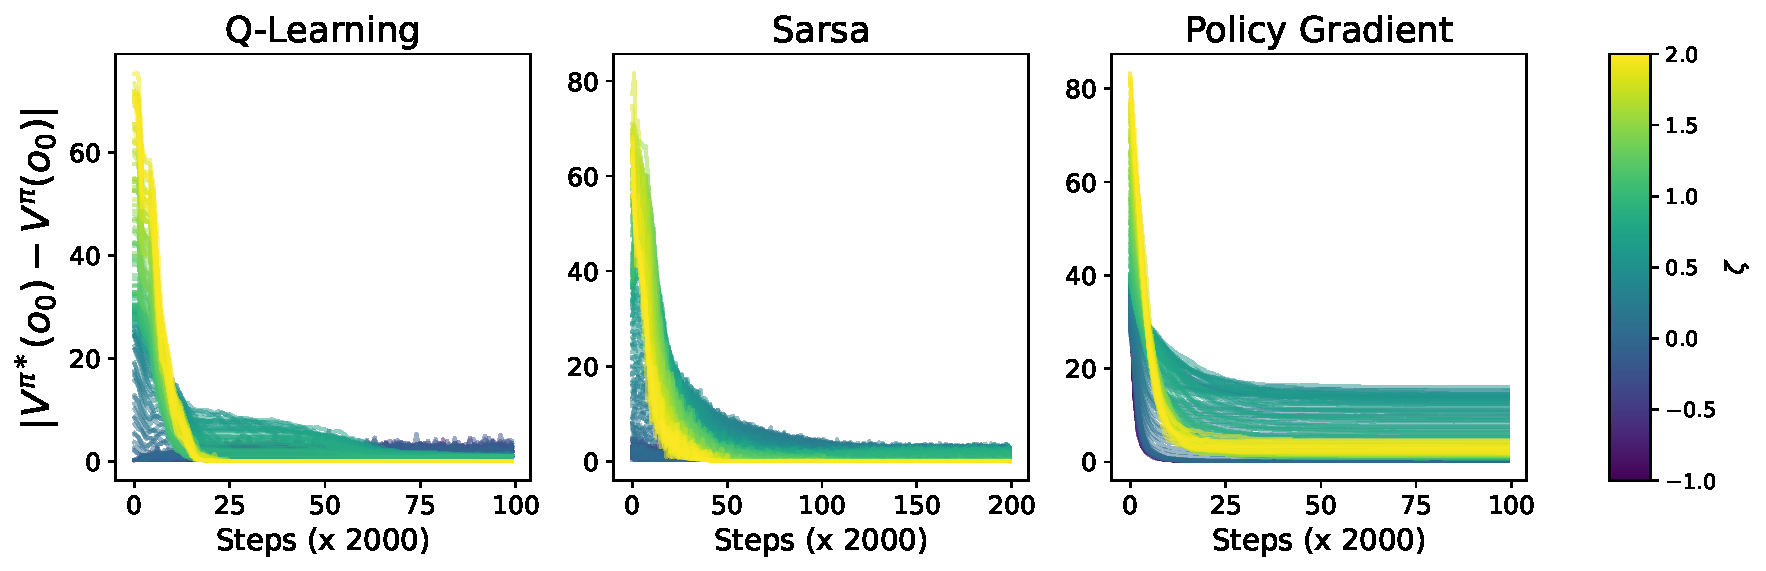
\includegraphics[width=1\textwidth]{images/images_part1/learning_curves_classif.pdf}
    \caption{}\label{fig:rl-classif-poibmdp}
\end{figure}

\begin{figure}
    \centering
    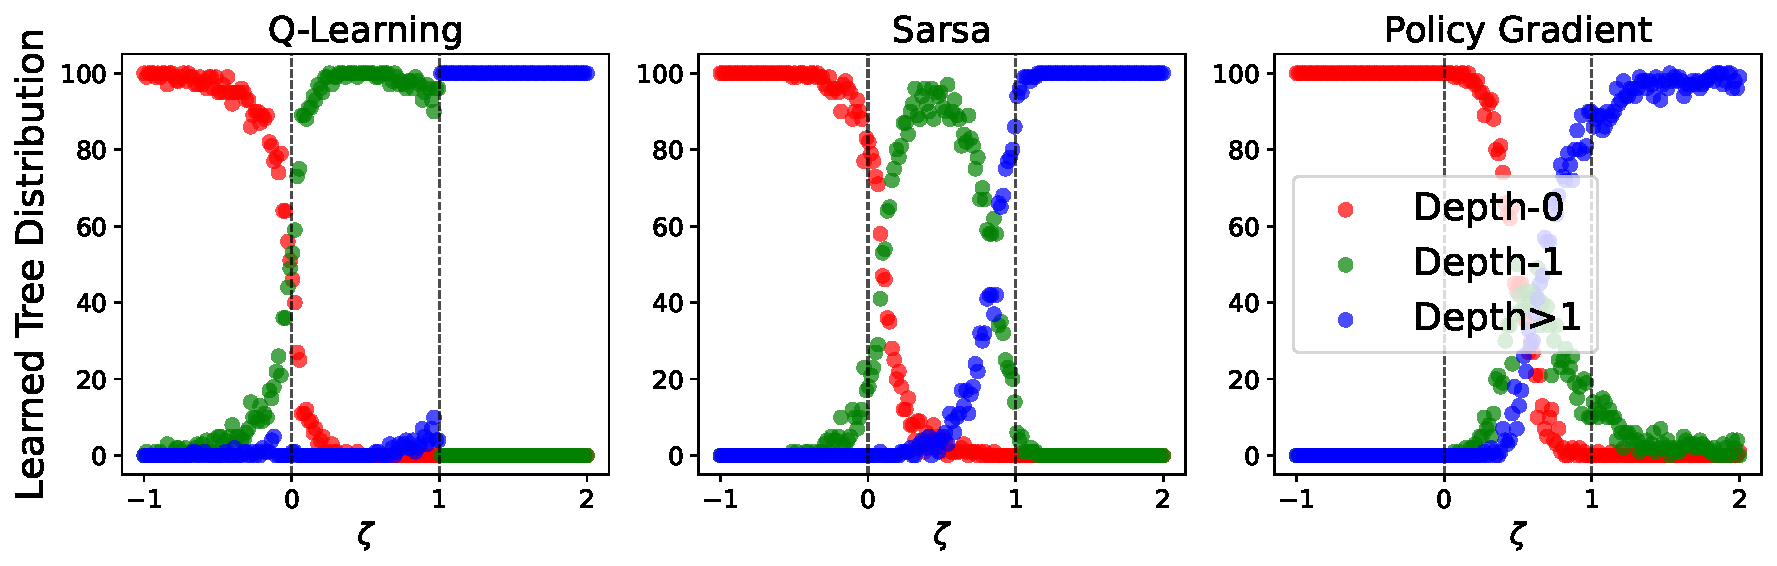
\includegraphics[width=1\textwidth]{images/images_part1/tree_distributions_classif.pdf}
    \caption{}\label{fig:tree-distrib-classif-poibmdp}
\end{figure}

Fortunately this time, compared to general POIBMDPs, RL can be used to retrieve optimal policies in classification POIBMDPs equivalent to decision tree classifiers.
We observe on Figure (cite) that both Q-learning and Sarsa consistently minimize the sub-optimality gap. 
Hence they are able to retrieve the optimal detph-1 decision tree classifier from Figure (cite).

In this part of the manuscript, we have highlighted the challenges of directly learning decision tree policies for MDPs.
In particular in Chapter (cite), we showed that when we tried to reproduce existing baselines for direct RL of decision tree policies (cite), those often performed worse in terms of RL objective than the indirect approaches VIPER or Dagger even though the latter optimize the imitation learning objective (cite).

We further analyzed the failure mode of direct learning of decision tree policies by making connexions with POMDPs.
In Chapter (cite), we showed that learning decision tree policies for MDPs that optimize the RL objective could be explicitely formulated as learning a deterministic partially observable (also known as memoryless or reactive) policy in a specific POMDP that we called POIBMDP.
We showed that both RL and asymmetric RL, a class of algorithms specifically designed for POMDPs, were unable to consistently retrieve optimal depth 1 decision tree policy for a very small $2\times2$ grid world.

Finally, in this Chapter we showed that RL in fully observable POIBMDPs, i.e. POIBMDPs that are just MDPs, could retrieve optimal decision tree policies, we conjecture that most of the difficulty for the general POIBMDP case arise from the partial observability.
This provides one clear avenue for future research: developing algorithm tailored for POIBMDPs.

However it is hard to encourage such research when indirect methods like VIPER or Dagger already optimize the RL objective pretty well and often require few samples if an neural network expert policy is already available.

In the next part of this manuscript, we extend the ideas of classification POIBMDPs (cite) and show how to design competitive decision tree induciton algorithms for the supervised learning objective using techniques from MDPs.

